%; whizzy paragraph -pdf xpdf -latex ./whizzypdfptex.sh
%; whizzy-paragraph "^\\\\begin{frame}"
% latex beamer presentation.
% platex, latex-beamer でコンパイルすることを想定。 

%     Tokyo Debian Meeting resources
%     Copyright (C) 2009 Junichi Uekawa
%     Copyright (C) 2010 Nobuhiro Iwamatsu

%     This program is free software; you can redistribute it and/or modify
%     it under the terms of the GNU General Public License as published by
%     the Free Software Foundation; either version 2 of the License, or
%     (at your option) any later version.

%     This program is distributed in the hope that it will be useful,
%     but WITHOUT ANY WARRANTY; without even the implied warranty of
%     MERCHANTABILITY or FITNESS FOR A PARTICULAR PURPOSE.  See the
%     GNU General Public License for more details.

%     You should have received a copy of the GNU General Public License
%     along with this program; if not, write to the Free Software
%     Foundation, Inc., 51 Franklin St, Fifth Floor, Boston, MA  02110-1301 USA

\documentclass[cjk,dvipdfmx,12pt]{beamer}
\usetheme{Tokyo}
\usepackage{monthlypresentation}
%  preview (shell-command (concat "evince " (replace-regexp-in-string "tex$" "pdf"(buffer-file-name)) "&"))
%  presentation (shell-command (concat "xpdf -fullscreen " (replace-regexp-in-string "tex$" "pdf"(buffer-file-name)) "&"))
%  presentation (shell-command (concat "evince " (replace-regexp-in-string "tex$" "pdf"(buffer-file-name)) "&"))

%http://www.naney.org/diki/dk/hyperref.html
%日本語EUC系環境の時
\AtBeginDvi{\special{pdf:tounicode EUC-UCS2}}
%シフトJIS系環境の時
%\AtBeginDvi{\special{pdf:tounicode 90ms-RKSJ-UCS2}}

\title{東京エリア Debian 勉強会 \& Debian 温泉}
\subtitle{資料}
\author{前田 耕平 mkouhei@debian.or.jp\\IRC nick: mkouhei}
\date{2010年02月20,21日}
\logo{
\includegraphics[width=8cm]{image200607/openlogo-light.eps}}

\begin{document}

\frame{\titlepage{}}

\emtext{設営準備にご協力ください}


\begin{frame}
 \frametitle{勉強会の連絡事項}
\begin{minipage}[t]{0.45\hsize}
  \begin{itemize}
   \item 注意事項(両日共通)
	 \begin{itemize}
	  \item 飲食OK
	  \item ゴミは持ち帰り
	  \item 終了後掃除
	 \end{itemize}
  \end{itemize}

\end{minipage} 
\begin{minipage}[t]{0.45\hsize}
 \begin{itemize}
  \item 本日の勉強会終了後、お茶会を行います
  \item チェックインは20時まで
 \end{itemize}
\end{minipage}
\end{frame}

\section{}
\begin{frame}
 \frametitle{Agenda}
 \begin{minipage}[t]{0.45\hsize}
  \begin{itemize}
   \item 本日は13:00-17:00です
   \item 事前課題紹介
   \item Debian の紹介
   \item OCaml環境で開発する関数型言語インタプリタ
  \end{itemize}
 \end{minipage} 
 \begin{minipage}[t]{0.45\hsize}
  \begin{itemize}
   \item 明日は9:00-13:00の予定です。
   \item ブート方法が変わるよ
   \item プログラミング言語 Yadorigi
   \item 東京エリアDebian勉強会予約システムの構想
  \end{itemize}
 \end{minipage}
\end{frame}

\begin{frame}{Hack Cafe}
 毎週火曜日、週に一回東京のどっかのカフェでハック。\\
 \url{http://twitter.com/debian_hackcafe}\\
 関西でも始めたようです。
\end{frame}

\emtext{事前課題}

\begin{frame}{事前課題}
\begin{enumerate}
 \item Debian について現在知っていることを教えてください。
 \item Debian について知りたいとおもっていることを教えてください。
 \item Debianを使う理由を挙げてください。
\end{enumerate}
\end{frame}

{\footnotesize
\begin{prework}{ �����ϥ� }
\begin{enumerate}
\item �ϻϼԤ� Ian ����Ȥ��κ� Debra �����̾������̿̾���줿�� 
\item ���äѤ����ꤹ���ơ�������ˤ����ޤ�ʤ���
\item ���֤���ͳ�ϡ���ʬ�����ޤΤ��㤯�����餫�ʤ���
\end{enumerate}
\end{prework}
\begin{prework}{ emasaka }
\begin{enumerate}
\setcounter{enumi}{2}
\item �Ȥˤ�����������Υѥå��������鹽��������ǡ����뤤��ɬ�פ˱�����
      �ѥå��������ɲä��ơ��ʤ����Ĥ������ٰ¿����ơ����Ӥ˹�ä�������
      ����Ȥ������
\end{enumerate}
\end{prework}
\begin{prework}{ henrich }
\begin{enumerate}
\item dis���ʤ���⤬��Ф�򵤤ʥץ��������ȤǤ���
\item �ץ��������ȥ꡼�����γ�ư�����β����Ƥ�Ρ���
\item �ֱ郎���ä�����פǤ� :)
\end{enumerate}
\end{prework}
\begin{prework}{ mkouhei }
\begin{enumerate}
\setcounter{enumi}{2}
\item ʣ���Υ������ƥ�����Υޥ���򡢤��ΰ㤤�򵤤ˤ��������ѤǤ���ѥ�
      �����������ƥब���������뤿��Ǥ����Ȥ��Ϥ᤿���ä����Ǥ⤢��ޤ���
      �����ǻȤäƤ���Τ����Ǥ�5����Ǥ���
\end{enumerate}
\end{prework}
\begin{prework}{ ����(yy\_y\_ja\_jp) }
\begin{enumerate}
\setcounter{enumi}{2}
\item DFSG�����뤫�顥\&�ѥå������󥰥����ƥबͥ��Ƥ��뤫�顥�Ǥ��͡�
\end{enumerate}
\end{prework}
\begin{prework}{ ������ }
\begin{enumerate}
\setcounter{enumi}{2}
\item ������������ۤΥѥå��������������ƥ�˽в�ä��Ȼפäư��衢���äȻȤäƤޤ���
\end{enumerate}
\end{prework}

}
\emtext{Debian の紹介}
\emtext{OCaml環境で開発する関数型言語インタプリタ}
\emtext{ブート方法が変わるよ}




\emtext{要点}

\begin{frame}
 \frametitle{Squeeze から変更される}
 \begin{itemize}
  \item sysvinit から upstart に変わる
  \item まずは互換モードから
  \item 今んとこ getty の挙動がかなり怪しい
 \end{itemize}
\end{frame}

\emtext{以上だけど、何か?}

\begin{frame}{upstart って何?}
 \begin{itemize}
  \item sysvinit の後継
  \item イベントドリブンのブートの仕組み
  \item cron, at, inetd なども最終的にはこれにするのが目標
 \end{itemize}
\end{frame}

\begin{frame}{そもそも sysvinit とは}
 \begin{itemize}
  \item システムブート時に各種プロセスを起動させる
  \item コンソールのログイン画面もこれ経由
  \item システム停止時のプロセスの終了とか
 \end{itemize}
\end{frame}

\begin{frame}{システムブートの大まかな流れ}
\begin{center}
\includegraphics[height=0.78\hsize]{image201002/sysvinit.eps}
\end{center}
\end{frame}

\begin{frame}{upstart に切り替える動機}
\begin{itemize}
 \item sysvinit って遅いよね(?)
 \item USB のプラグアンドプレイがうまく行かないよね(?)
 \item sysvinit ってもう古いよね。
\end{itemize}
\end{frame}

\emtext{ということらしいんですが、本当?}

\begin{frame}{他のディストロでは既に}
\begin{itemize}
 \item Ubuntu はもちろん、Fedora も既に
 \item Google の Chrome OS そうらしい
 \item Ubuntu 9.10 はネイティブモードらしい
\end{itemize}
\end{frame}

\begin{frame}{一方、Debian では}
\begin{itemize}
 \item Squeeze から変わるらしいけど、現状はまだ sysvinit がデフォル
       ト
 \item 互換モードなので、p.34 6.2.1のように大部分は変わらない
 \item なんだけど、getty の設定は inittab ではなく、/etc/init/ttyN.conf
       で行うように
 \item Ctrl+Alt+Del の設定も/etc/init/control-alt-delete.confに
\end{itemize}
\end{frame}

\begin{frame}{ネイティブモードだと全てイベントドリブン}
\begin{center}
\includegraphics[height=0.78\hsize]{image201002/states.eps}
\end{center}
\end{frame}

\emtext{取り合えず upstart へ}

\begin{frame}[containsverbatim]{Squeeze/Sidには入っている}
 パッケージでの導入は割と簡単。
\begin{commandline}
$ sudo apt-get install upstart
パッケージリストを読み込んでいます... 完了
依存関係ツリーを作成しています                
状態情報を読み取っています... 完了
以下の特別パッケージがインストールされます:
  dbus libdbus-1-3 libexpat1
提案パッケージ:
  dbus-x11
以下のパッケージは「削除」されます:
  sysvinit
以下のパッケージが新たにインストールされます:
  dbus libdbus-1-3 libexpat1 upstart
警告: 以下の不可欠パッケージが削除されます。
何をしようとしているか本当にわかっていない場合は、実行してはいけません!
  sysvinit
アップグレード: 0 個、新規インストール: 4 個、削除: 1 個、保留: 9 個。
1,005kB のアーカイブを取得する必要があります。
この操作後に追加で 2,105kB のディスク容量が消費されます。
重大な問題を引き起こす可能性のあることをしようとしています。
続行するには、'Yes, do as I say!' というフレーズをタイプしてください。
 ?] Yes, do as I say!
\end{commandline}
\end{frame}

\begin{frame}[containsverbatim]{getty ちゃんと動かないじゃん!}
「先生、ログイン画面が表示されません!」
\begin{commandline}
init: tty4 main process (239) terminated with status 1
init: tty4 main process ended, respawning
init: tty5 main process (241) terminated with status 1
init: tty5 main process ended, respawning
init: tty2 main process (242) terminated with status 1
init: tty2 main process ended, respawning
(end less)
\end{commandline}

…ssh 経由のターミナルログインはできるので、まあサーバとしては使えます。
\end{frame}

\emtext{大丈夫か?}

\begin{frame}{とはいえ決まったことなので}
 \begin{itemize}
  \item Squeeze/Sid で人柱に協力しませう
  \item Sid 使っていない人はまず Sid にしてみませう
  \item 仮想マシンで試すのがよいせう
 \end{itemize}
\end{frame}

\emtext{プログラミング言語 Yadorigi}
\emtext{東京エリアDebian勉強会予約システムの構想}

\begin{frame}{}
 
 東京エリアDebian勉強会予約システムの構想

 上川純一
 
\end{frame}


\begin{frame}{Debian 勉強会予約システム}
 \begin{itemize}
 \item イベントの主催者が簡便に登録情報を設定することができること。
 \item イベントの主催者が事前課題を設定し、回答を簡単に収集することがで
       きること。
 \item イベントの主催者が簡単に参加人数を確認することができること。
 \item イベントの主催者が新規参加者の情報を迅速に確認できること。
 \item イベントの主催者が参加者に直接連絡がとれる手段があること。
 \item 参加者が簡単に事前課題もあわせて登録できること。
 \item 参加者がイベント参加をキャンセルする方法があること。
 \item 参加者が参加しているイベントを把握する方法があること。
\end{itemize}
\end{frame}

\begin{frame}{}

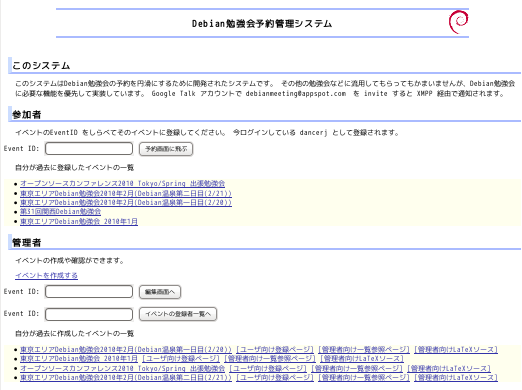
\includegraphics[width=1\hsize]{image201002/debianmeeting-screenshot.png}

\end{frame}

\begin{frame}{Google App Engine for Python}
\begin{itemize}
 \item Python Django ベースのウェブアプリケーションフレームワークホスティ
       ング環境
 \item App Engine 環境で動作するため、Djangosそのままでは動作せず、修正
       が必要。
\end{itemize}
\end{frame}

\begin{frame}[containsverbatim]{Google App Engine SDK をインストール}
\begin{commandline}
 # apt-get install unzip python python-webtest python-yaml
\end{commandline}

ソースはDebian勉強会資料の utils/gae 以下。

\end{frame}

\begin{frame}[containsverbatim]{ローカルで起動}
\begin{commandline}
$ ../../google_appengine/dev_appserver.py
\end{commandline}
% $ -- for emacs

\url{http://localhost:8080/} でサービス提供
\url{http://localhost:8080/_ah/admin} で管理画面。

\end{frame}

\begin{frame}{ログイン画面}


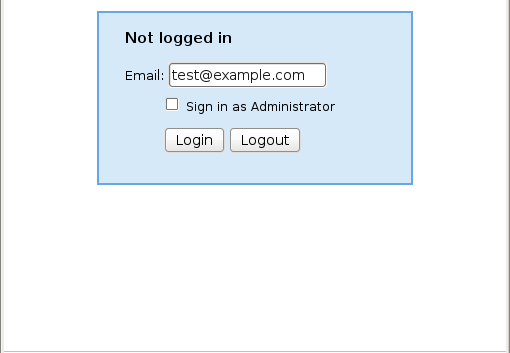
\includegraphics[width=6cm]{image201002/gae-local-login.png}

ローカルで立ち上げたデバッグ用のインスタンスに対しては管理者としてログインするかどうかが選択できる。
\end{frame}

\begin{frame}{管理画面}

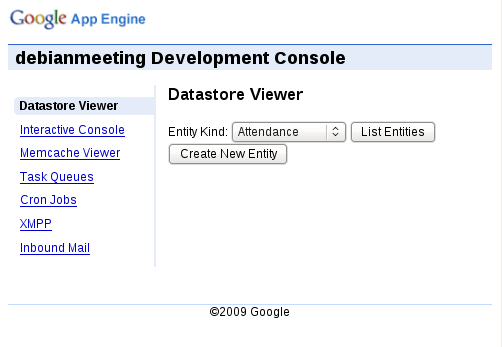
\includegraphics[width=6cm]{image201002/debianmeeting-localhost-admin.png}

管理ツールもあります。
データストアの中身などがのぞけます。
\end{frame}

\begin{frame}[containsverbatim]{アップロード}

サーバにアップロード
 \begin{commandline}
$ ../../google_appengine/appcfg.py update
Initiating update.
Email: dancerj@gmail.com
Password for dancerj@gmail.com: 
 \end{commandline}
\url{http://debianmeeting.appspot.com} でサービス提供
\end{frame}

\begin{frame}[containsverbatim]{テストの実行}
 AppEngine のフレームワークではテスト用のツールが提供されていないので、
 外部ツールを利用する。
 gaeunitなどの選択肢がある。

 python-webtest を活用してテストする。
 \begin{commandline}
$ PYTHONPATH=../../google_appengine:../../google_appengine/lib/django/ \
 python testSystem.py
 \end{commandline}
\end{frame}


\begin{frame}{データベースの構成}
\begin{minipage}{0.4\hsize}
 \begin{itemize}
 \item Event
 \item Attendance
 \item User
 \end{itemize}
\end{minipage}
\begin{minipage}{0.5\hsize}
\begin{itemize}
 \item Event に複数の Attendance がある
 \item ユーザには複数の Attendance がある
\end{itemize}
\end{minipage}
\end{frame}


\begin{frame}[containsverbatim]{データベースの構成:Event}
イベントを管理する

\begin{commandline}
 class Event(db.Model):
    eventid = db.StringProperty()
    owner = db.UserProperty() # the creator is the owner
    owners_email = db.StringListProperty() # allow owner emails to be added if possible
    title = db.StringProperty()
    location = db.StringProperty(multiline=True)
    content = db.StringProperty(multiline=True)
    content_url = db.StringProperty()
    prework = db.StringProperty(multiline=True)
    event_date = db.StringProperty()
    timestamp = db.DateTimeProperty(auto_now_add=True)
    capacity = db.IntegerProperty() # the number of possible people attending the meeting
\end{commandline}
\end{frame}

\begin{frame}[containsverbatim]{データベースの構成:Attendance}
イベントに対しての出席を管理する

\begin{commandline}
class Attendance(db.Model):
    eventid = db.StringProperty()
    user = db.UserProperty()
    user_realname = db.StringProperty() # keep a cache of last realname entry.
    prework = db.StringProperty(multiline=True) # obsolete, but used in initial version
    prework_text = db.TextProperty() # Used everywhere, populate from prework if available.
    attend = db.BooleanProperty()
    enkai_attend = db.BooleanProperty()
    timestamp = db.DateTimeProperty(auto_now_add=True)
\end{commandline}
\end{frame}

\begin{frame}[containsverbatim]{データベースの構成:UserRealName}
ユーザの名前を管理する

\begin{commandline}
class UserRealname(db.Model):
    """Backup of user realname configuration so that user doesn't have to reenter that information."""
    user = db.UserProperty()
    realname = db.StringProperty()
    timestamp = db.DateTimeProperty(auto_now_add=True)
\end{commandline}
\end{frame}

\begin{frame}{ソースツリーの構成}
\begin{itemize}
 \item \url{debianmeeting.py}: どのページがどのコードを呼び出すのかとい
       う部分を管理しているコードです。あと、どこに入れるのか迷ったコー
       ドもここにあるかも。
 \item \url{admin_event.py}: 主催者のイベントの管理関連のコードです。
 \item \url{user_registration.py}: ユーザの登録関連のコードです。
 \item \url{webapp_generic.py}: とりあえず共通のロジックを定義しています。
       POST と GET を同じように扱うためのコードなどが入っています。
 \item \url{schema.py}: データストアのスキーマが定義されています。
 \item \url{send_notification.py}: メール送信とXMPP送信ロジックが記述さ
       れています。
 \item \url{testSystem.py}: ユニットテストです。
\end{itemize}
\end{frame}

\begin{frame}{ウェブページの遷移}

\includegraphics[width=1\hsize]{image201001/debian-reservation-flow.eps}
 
\end{frame}

\begin{frame}{次回の勉強会}

\begin{itemize}
 \item 2010年2月27日: OSC Tokyo 2010Spring
 \item 明星大学にて
\end{itemize}
 
\end{frame}

\end{document}

;;; Local Variables: ***
;;; outline-regexp: "\\([ 	]*\\\\\\(documentstyle\\|documentclass\\|emtext\\|section\\|begin{frame}\\)\\*?[ 	]*[[{]\\|[]+\\)" ***
;;; End: ***
